\documentclass[11pt,a4paper]{article}

\usepackage[utf8]{inputenc}
\usepackage[T1]{fontenc}
%\usepackage[cm]{fullpage}
\usepackage[top=1.5cm,bottom=1.5cm,margin=2.5cm]{geometry}
\usepackage[french]{babel}

\usepackage{graphicx}
\graphicspath{{images/}}

\usepackage{amsmath,amsmath,amssymb}
\usepackage{mathtools}

\usepackage{algorithmic}
\usepackage[lined,commentsnumbered,boxed]{algorithm2e}
\usepackage{listings}

\usepackage{xcolor}

\usepackage{appendix}
\def\appendixpagename{Annexes}
\def\appendixtocname{Annexes}

%\usepackage{float}

\newcommand{\HRule}{\rule{\linewidth}{0.5mm}}

\providecommand{\keywords}[1]{\textbf{\textit{Mots-clés:}} #1}

\usepackage{url}
\usepackage[pdfusetitle]{hyperref}


\title{Le nom de votre projet}
\author{Prénom1 NOM1\\Prénom2 NOM2\\Prénom3 NOM3}
\def\tuteur{Prénom NOM}

\begin{document}

\begin{titlepage}
\begin{center}

{\LARGE\scshape
École nationale de la statistique

et de l'analyse de l'information}

\vspace{5mm}

\includegraphics[width=0.4\textwidth]{ensai_logo}
\vspace{1cm}

\textsc{\LARGE Projet de Traitement de Données (1AINF06)}

\vspace{0.5cm}

{\huge
\HRule

\vspace{0.4cm}

\bfseries\makeatletter\@title\makeatother

\vspace{0.4cm}

\HRule}

\vspace{1.5cm}

% Author and supervisor

\begin{flushleft}
    \Large
    \emph{Groupe:}

    \scshape\makeatletter\@author\makeatother
\end{flushleft}

\begin{flushright}
    \Large
    \emph{Tuteur:}

    \textsc{\tuteur}

    \emph{Responsable du Cours:}

    \textsc{Benjamin GIRAULT}
\end{flushright}


\vfill
{\large Année 2022}
\end{center}
\end{titlepage}


\begin{abstract}
  \emph{Mettez ici le résumé de ce travail (environ 10-15 lignes).}

  Nous présentons dans ce rapport l'étude sur les données de quelque chose \dots
  On va présenter tout d'abord ... puis, ...
\end{abstract}

%\tableofcontents

\section{Introduction}

Présentez le projet, vos objectifs (les grandes lignes seulement) et les méthodes utilisées.

%\begin{figure}[tb]
%\includegraphics[width=\textwidth]{projet_py_1er_annee}
%\caption{\label{fig:1}}
%\end{figure}

\section{Cahier des charges}

Décrire \emph{la maquette} de votre application: que doit-il se passer lors de l'exécution?

Construisez des diagrammes de votre application décrivant les fonctionnalités que vous coderez (diagramme d'état / diagramme d'activité et/ou diagramme de cas d'utilisation).

\subsection{Diagramme de cas d'utilisation}

La \autoref{fig:cas_utilisation} présente le diagramme de cas d'utilisation de notre projet.

\begin{figure}[tb]
  \centering
  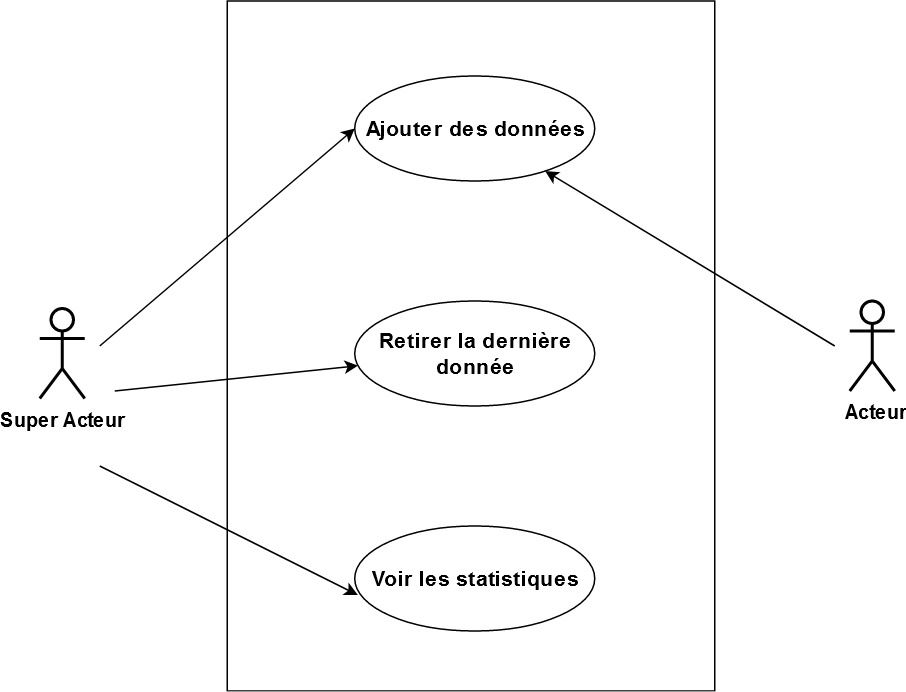
\includegraphics[width=0.9\linewidth]{diagramme_cas_utilisation}
  \caption{Diagramme de cas d'utilisation de \dots}
  \label{fig:cas_utilisation}
\end{figure}

\subsection{Diagramme(s) d'activité}

La \autoref{fig:activite} présente le diagramme d'activité de notre projet.

\begin{figure}[tb]
  \centering
  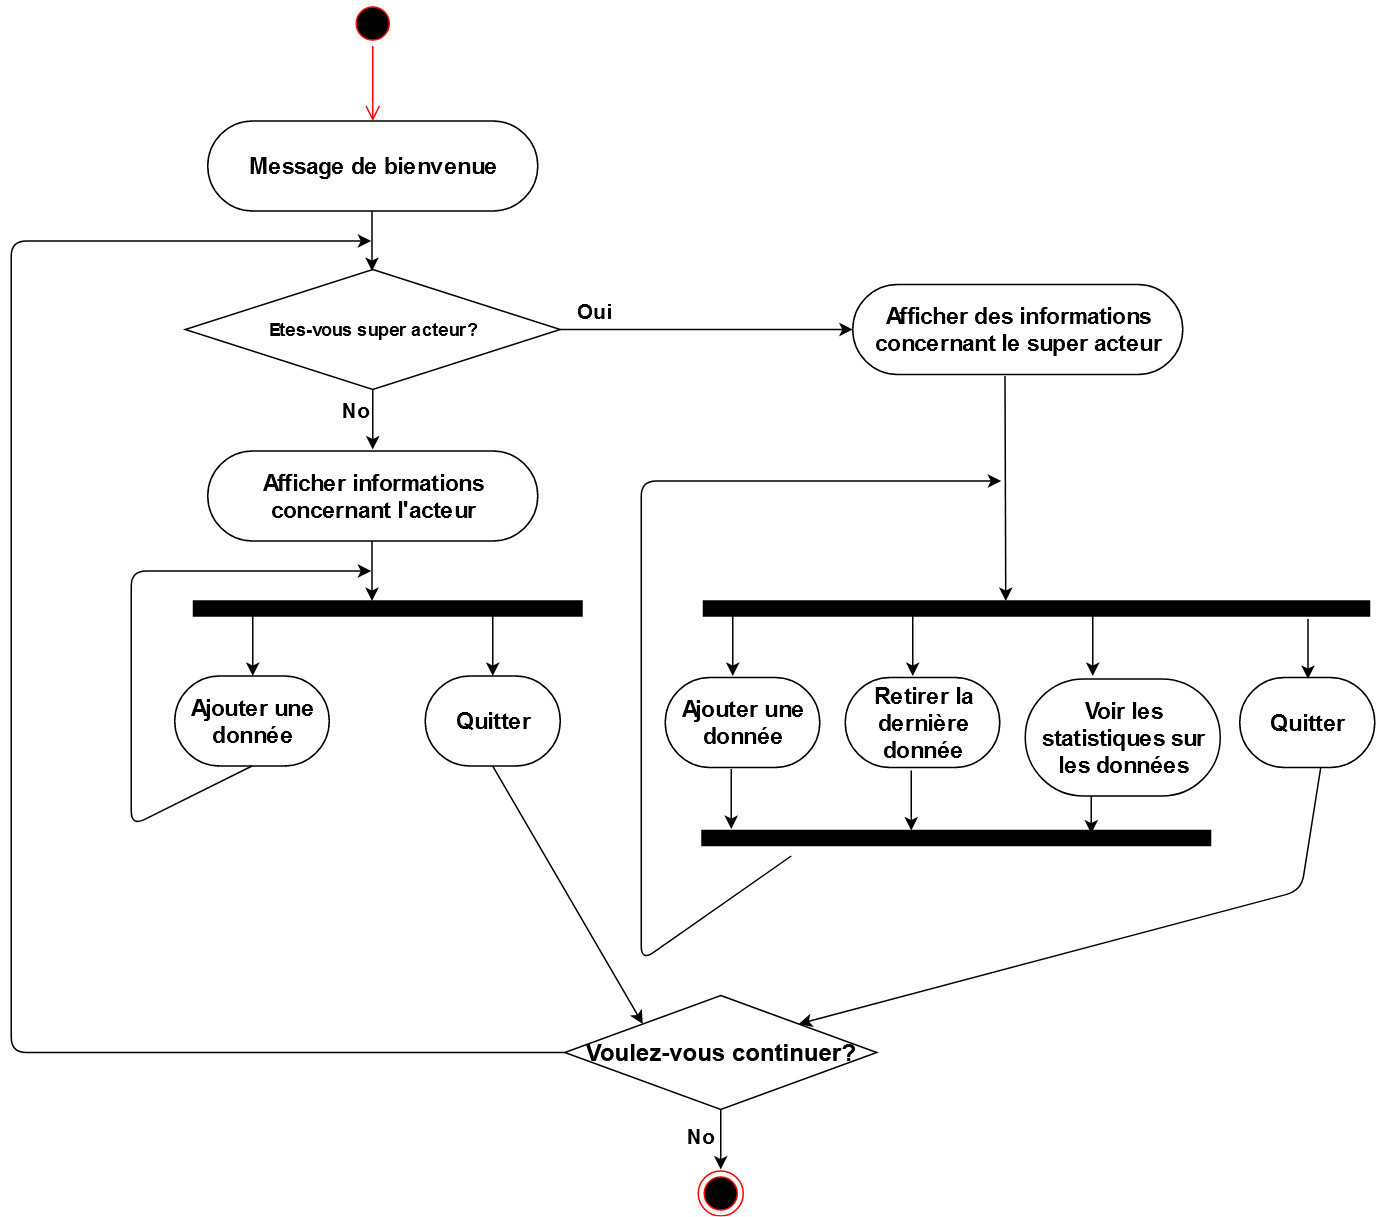
\includegraphics[width=\linewidth]{diagramme_activite}
  \caption{Diagramme d'activité}
  \label{fig:activite}
\end{figure}

\section{Architecture de l'application}

\subsection{Architecture de l'archive}

Présentez le contenu de votre projet: dossiers, fichiers et le rôle de chaque dossier/fichier ainsi que le type de chaque fichier (txt, json, jpg, etc.)
Présentez les \emph{packages} et les modules.

\subsection{Architecture du code: fonctions}

Présentez les fonctions (leur signature) ainsi que leurs fonctionnalités dans chaque module (les signatures des fonctions et leur documentation pourront être générées automatiquement et placées dans une annexe référencée dans cette section, mais seulement si le code est correctement documenté).
Attention, les méthodes de classe ne sont pas à présenter dans cette section.
Si vous n'avez aucune fonction, vous pouvez supprimer cette section.

\subsection{Architecture du code: classes}

Présentez les classes, les méthodes, et les attributs de chaque classe.
Vous pouvez générer automatiquement cette section à partir de la documentation du code (si elle est complète), et la placer en annexe.

\subsection{Diagramme de classe}

La \autoref{fig:diagramme_classe} présente le diagramme de classe de notre projet.

\begin{figure}[tb]
  \centering
  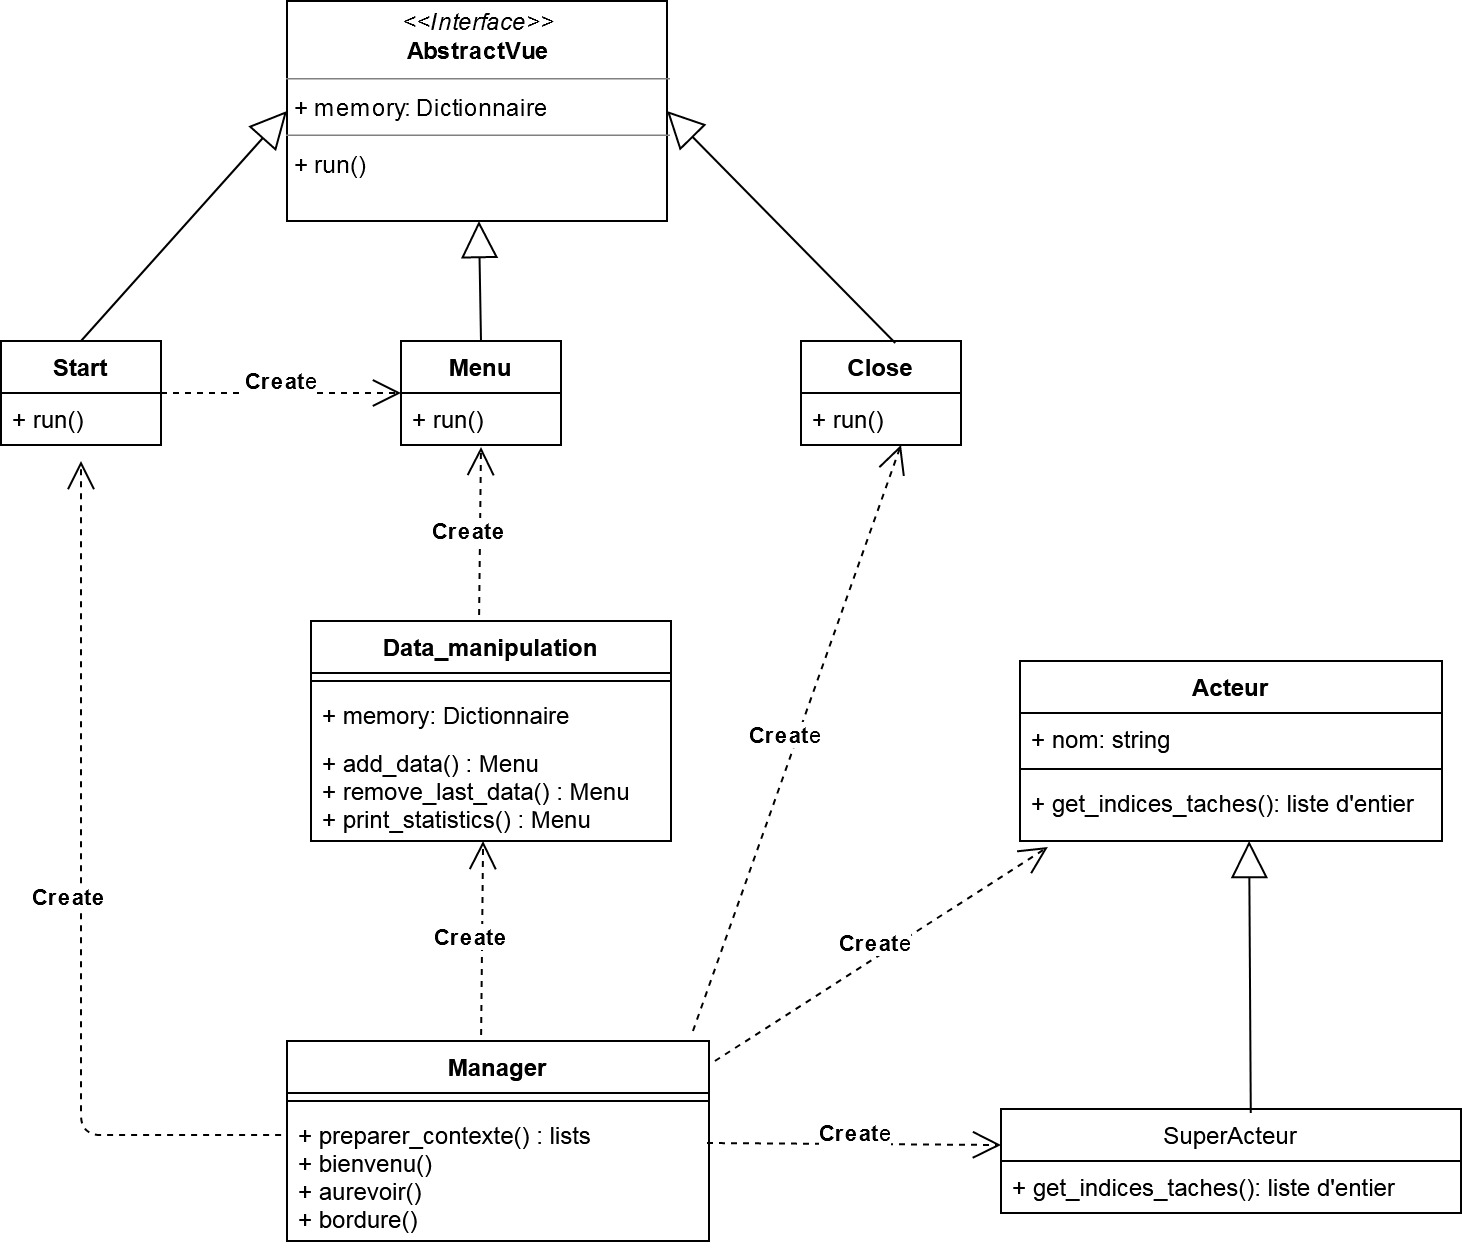
\includegraphics[width=\linewidth]{diagramme_classe}
  \caption{Diagramme de classe}
  \label{fig:diagramme_classe}
\end{figure}

\section{Gestion des données}

Comment avez-vous géré les données: 
\begin{itemize}
    \item Quel type de stockage? liste, dictionnaire ou autre et pourquoi ce choix?
    \item Comment ajouter / modifier / enlever des données?
    \item Y a-t-il un enregistrement de données sur le disque? et si oui, pourquoi et comment?
    \item etc.
\end{itemize}

\section{Tests}

\subsection{Tests unitaires}

Listez les fonctionnalités des classes que vous avez testées.

\subsection{Tests fonctionnels}

Cette section concerne les tests en situation réelle de votre programme: se comporte-t-il correctement lorsque vous le lancez avec les données?
Expliquez les tests que vous avez fait.
En particulier, expliquez les questions d'analyse de données vous avez exécutées et quelles fonctionnalités de votre programme elles testent.

% \section{Résultats}
% 
% Illustrez vos résultats ici avec des commentaires.

\section{Répartition du travail}

Qui fait quoi, ce que vous avez appris.

\section{Conclusion et perspectives}

Résumez ce que vous avez fait, présentez les résultats obtenus, donnez votre conclusion et vos perspectives\dots

% Décommentez ci-dessous si vous avez besoin d'une bibliographie
% \bibliographystyle{apalike}
% \bibliography{bibliography}

\appendix

\appendixpage
\addappheadtotoc

\section{Documentation}

Présentez la documentation générée automatiquement à partir des commentaires dans le code, si vous en avez.

\end{document}
